\documentclass[10pt]{article}
\usepackage[ngerman]{babel}
\usepackage[utf8]{inputenc}
\usepackage[T1]{fontenc}
\usepackage{amsmath}
\usepackage{amsfonts}
\usepackage{amssymb}
\usepackage[version=4]{mhchem}
\usepackage{stmaryrd}
\usepackage{graphicx}
\usepackage[export]{adjustbox}
\graphicspath{ {./images/} }
\usepackage{bbold}

\title{Hauptprüfung Abiturprüfung 2021 - Leistungsfach }

\author{Alexander Schwarz\\
www.mathe-aufgaben.com}
\date{}


\begin{document}
\maketitle
 Baden-Württemberg\section*{Pflichtteil - Aufgabensatz 1}
Hilfsmittel: keine allgemeinbildende Gymnasien

August 2021

\section*{Aufgabe 1: (1 VP und 1,5 VP)}
Gegeben ist die Funktion $f$ mit $f(x)=e^{-2 x+1}+1$. Die Abbildung zeigt den Graphen $G_{f}$ sowie die Tangente an $G_{f}$ an der Stelle $x=\frac{1}{2}$.\\
a) Weisen Sie nach, dass diese Tangente die Steigung -2 hat.\\
b) Berechnen Sie den Flächeninhalt des Dreiecks, das diese Tangente mit den Koordinatenachsen einschließt.\\
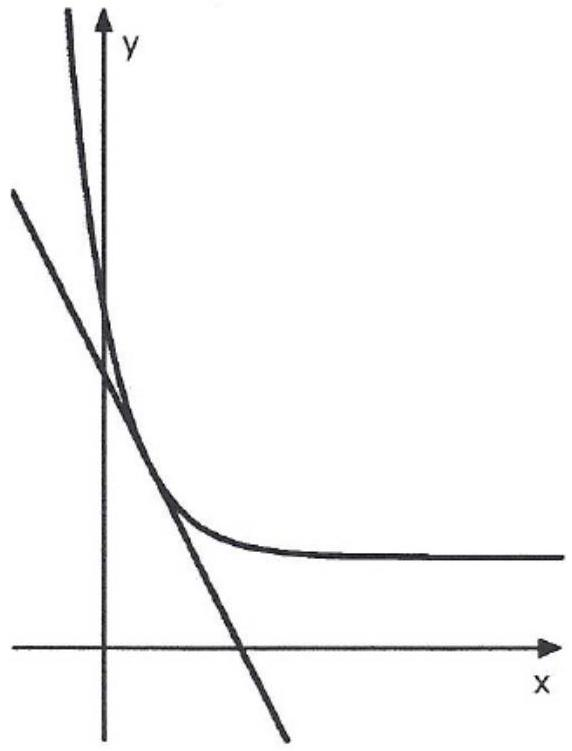
\includegraphics[max width=\textwidth, center]{2025_04_24_8c9697e05ae22baf56a2g-02(2)}

\section*{Aufgabe 2: (2,5 VP)}
Die Abbildung zeigt den Graphen der Funktion $f$ mit $f(x)=1+x^{2}$ sowie die Geraden $g: y=2$ und $\mathrm{h}: \mathrm{y}=5$.

Bestimmen Sie den Inhalt der markierten Fläche.\\
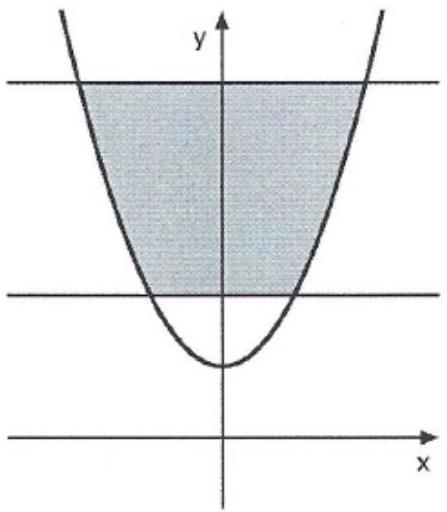
\includegraphics[max width=\textwidth, center]{2025_04_24_8c9697e05ae22baf56a2g-02}

\section*{Aufgabe 3: (1 VP und 1,5 VP)}
Gegeben sind die Funktionen $f$ und $g$ mit $f(x)=a+\frac{b}{x^{2}+c}$ und $g(x)=a+\frac{b}{(x+c)^{2}}$.\\
Die Abbildung zeigt den Graphen einer der beiden Funktionen sowie seine Asymptoten.\\
a) Begründen Sie , dass es sich bei dem abgebildeten Graphen nicht um den Graphen von $f$ handeln kann.\\
b) Bestimmen Sie für die Funktion g die\\
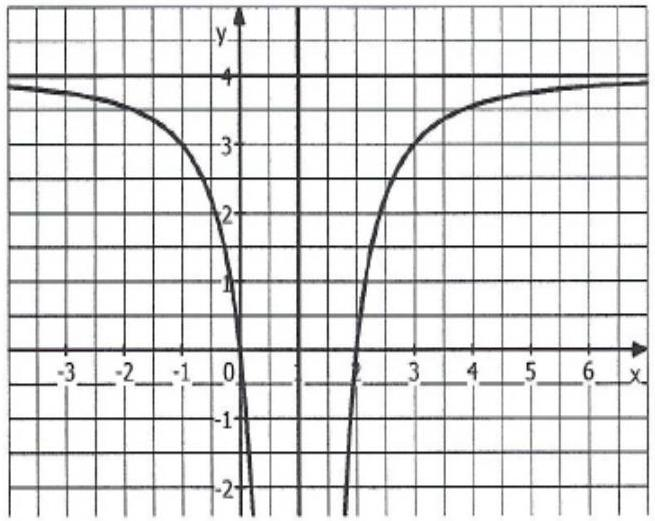
\includegraphics[max width=\textwidth]{2025_04_24_8c9697e05ae22baf56a2g-02(1)} Werte von $\mathrm{a}, \mathrm{b}$ und c .

\section*{Aufgabe 4: (1 VP und 1,5 VP)}
Die Abbildung zeigt den Graphen der Funktion $f$. Die Funktion $g$ ist gegeben durch $g(x)=f(x)+5 x$.\\
Entscheiden Sie jeweils, ob die folgenden Aussagen wahr oder falsch sind, und begründen Sie Ihre Entscheidung.\\
(1) Jede Stammfunktion von f besitzt im Intervall $[0,5 ; 4]$ genau ein lokales Maximum.\\
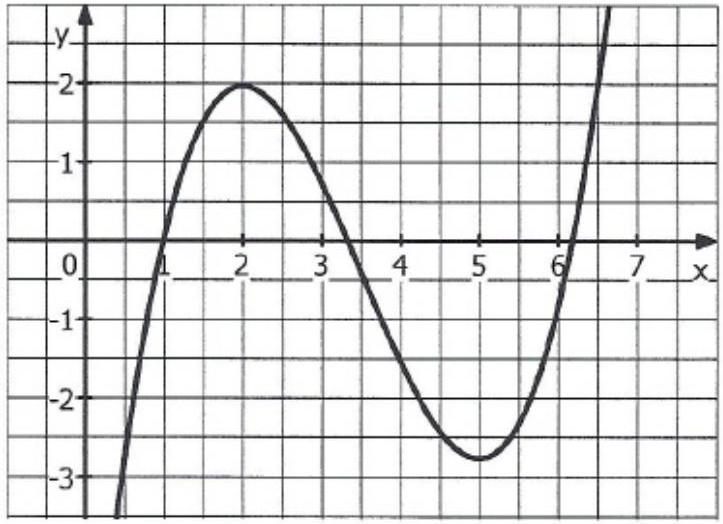
\includegraphics[max width=\textwidth, center]{2025_04_24_8c9697e05ae22baf56a2g-03}\\[0pt]
(2) Die Funktion g ist im Intervall [1;6] streng monoton steigend.

\section*{Aufgabe 5: (1 VP und 1,5 VP)}
Gegeben sind die Ebenen $E$ und $F$ sowie die Ebenenschar $G_{r}(r \in \mathbb{R})$.

E: $\quad x_{1}-5 x_{2}-2 x_{3}=6$\\
F: $2 x_{1}-x_{2}-x_{3}=3$\\
$\mathrm{G}_{\mathrm{r}}: \quad 9 \mathrm{x}_{2}+3 \mathrm{x}_{3}=\mathrm{r}+11$\\
a) Stellen Sie die Ebene $G_{7}$ in einem Koordinatensystem dar.\\
b) Für einen Wert von $r$ besitzen $E, F$ und $G_{r}$ eine gemeinsame Schnittgerade. Bestimmen Sie diesen Wert von r.

\section*{Aufgabe 6: (1 VP und 1,5 VP)}
Gegeben sind der Punkt $P(-1|1|-1)$ und die Gerade $g: \vec{x}=\left(\begin{array}{c}1 \\ -1 \\ 7\end{array}\right)+t \cdot\left(\begin{array}{c}1 \\ 2 \\ -2\end{array}\right), t \in \mathbb{R}$.\\
Der Punkt Q(3|3|3) liegt auf der Geraden g.\\
a) Zeigen Sie, dass $Q$ derjenige Punkt auf gist, der zu $P$ den kleinsten Abstand hat.\\
b) Bestimmen Sie die Koordinaten eines Punktes R auf der Geraden g , für den das Dreieck PQR den Flächeninhalt 27 hat.

\section*{Aufgabe 7: (2,5 VP)}
In einer Urne befinden sich vier schwarze und eine unbekannte Anzahl weißer Kugeln. Aus der Urne werden nacheinander zwei Kugeln mit Zurücklegen gezogen. Die Wahrscheinlichkeit, dabei zwei schwarze Kugeln zu ziehen, ist doppelt so groß wie die Wahrscheinlichkeit, zwei Kugeln unterschiedlicher Farbe zu ziehen. Bestimmen Sie die Gesamtzahl der Kugeln in der Urne.

\section*{Aufgabe 8: (1 VP und 1,5 VP)}
Die Abbildung stellt die Wahrscheinlichkeitsverteilung der Zufallsgröße $X$ dar.\\
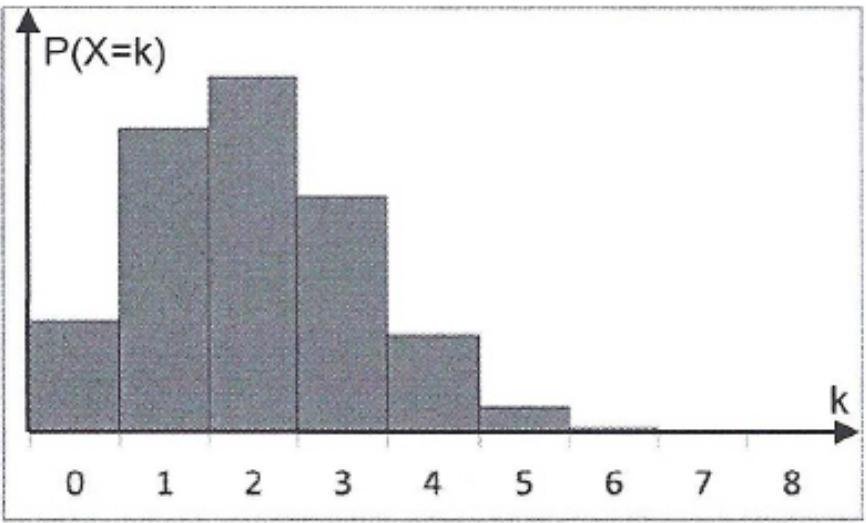
\includegraphics[max width=\textwidth, center]{2025_04_24_8c9697e05ae22baf56a2g-04}
a) 
Begründen Sie, dass $\mathrm{P}(\mathrm{X}=2)<0,5$ gilt.\\
b) Für eine binomialverteilte Zufallsgröße $Y$ mit den Parametern $n=8$ und $0<p<1$ gilt: $P(Y=1)=2 \cdot P(Y=0)$.\\
Berechnen Sie den Wert von $p$.

\section*{Aufgabe 1:}
a) $f(x)=e^{-2 x+1}+1$\\
$f^{\prime}(x)=-2 e^{-2 x+1}$\\
Steigung an der Stelle $x=\frac{1}{2}: f^{\prime}\left(\frac{1}{2}\right)=-2 \cdot e^{-2 \cdot \frac{1}{2}+1}=-2 \cdot e^{0}=-2$\\
Damit ist der Nachweis erbracht.\\
b) Zur Berechnung des Flächeninhalts muss die Gleichung der Tangente aufgestellt werden.

Ansatz für die Tangentengleichung: $y=f^{\prime}(u) \cdot(x-u)+f(u)$\\
Einsetzen der Berührstelle $u=\frac{1}{2}: y=f^{\prime}\left(\frac{1}{2}\right) \cdot\left(x-\frac{1}{2}\right)+f\left(\frac{1}{2}\right)$\\
Es gilt $f^{\prime}\left(\frac{1}{2}\right)=-2$ (Teilaufgabe a)) und $f\left(\frac{1}{2}\right)=e^{0}+1=2$\\
Tangentengleichung: $y=-2 \cdot\left(x-\frac{1}{2}\right)+2$ bzw. $y=-2 x+3$\\
Schnittpunkt der Tangente mit der y-Achse: $\mathrm{P}(0 \mid 3)$\\
Nullstelle der Tangente: $-2 x+3=0 \Leftrightarrow x=\frac{3}{2}$\\
Flächeninhalt des Dreiecks: $A=\frac{1}{2} \cdot \frac{3}{2} \cdot 3=\frac{9}{4}$ Flächeneinheiten

\section*{Aufgabe 2:}
Berechnung der Schnittpunkte der Parabel mit der Geraden y = 2:\\
$1+x^{2}=2 \Leftrightarrow x= \pm 1$\\
Es gilt $\mathrm{A}(-1 \mid 2)$ und $\mathrm{B}(1 \mid 2)$.\\
Berechnung der Schnittpunkte der Parabel mit der Geraden $y=5$ :\\
$1+x^{2}=5 \Leftrightarrow x= \pm 2$\\
Es gilt $C(-2 \mid 5)$ und $D(2 \mid 5)$.\\

Berechnung der Flächeninhalte $\mathrm{A} 1, \mathrm{~A} 2, \mathrm{~A} 3$ :\\
$\mathrm{A} 3=\int_{1}^{2}(5-f(x)) \mathrm{dx}=\int_{1}^{2}\left(4-x^{2}\right) \mathrm{dx}=\left[4 \mathrm{x}-\frac{1}{3} \mathrm{x}^{3}\right]_{1}^{2}=8-\frac{8}{3}-\left(4-\frac{1}{3}\right)=4-\frac{7}{3}=\frac{5}{3} \mathrm{FE}$\\
$\mathrm{A} 1=\mathrm{A} 3=\frac{5}{3} \mathrm{FE}$\\
$\mathrm{A} 2=2 \cdot 3=6 \mathrm{FE}$\\
Gesamte Fläche $=6 \mathrm{FE}+2 \cdot \frac{5}{3} \mathrm{FE}=\frac{28}{3} \mathrm{FE}$

\section*{Aufgabe 3:}
a) Die Funktion, die zu dem Graphen von f gehört besitzt eine Polstelle ohne Vorzeichenwechsel bei $x=1$.

Der Nenner des Funktionsterms von $f$ lautet $x^{2}+c$.\\
Fall $\mathrm{c}=0$ : Funktion f hat eine Polstelle ohne Vorzeichenwechsel bei $\mathrm{x}=0$.\\
Fall $c<0$ : Funktion $f$ hat zwei Pollstellen mit Vorzeichenwechsel bei $x= \pm \sqrt{-c}$.\\
Fall c > 0: Funktion f hat keine Polstelle.\\
Keiner der Fälle passt zu dem abgebildeten Graphen.\\
Eine andere Argumentation:\\
Das Schaubild von $f$ ist symmetrisch zur $y$-Achse, da $f(-x)=f(x)$ gilt.\\
Das abgebildete Schaubild ist nicht symmetrisch zur y-Achse.\\
b) $g(x)=a+\frac{b}{(x+c)^{2}}$

Aufgrund der Polstelle $\mathrm{x}=1$ ist $\mathrm{c}=-1$.\\
Die waagrechte Asymptote ist $\mathrm{y}=4$. Daraus folgt $\mathrm{a}=4$.\\
Zwischenergebnis: $g(x)=4+\frac{b}{(x-1)^{2}}$\\
Der Graph verläuft durch den Punkt $\mathrm{O}(0 \mid 0)$.\\
Einsetzen des Ursprungs in die Funktion: $0=4+\frac{\mathrm{b}}{(-1)^{2}} \Leftrightarrow b=-4$\\
$g(x)=4+\frac{-4}{(x-1)^{2}}$

\section*{Aufgabe 4:}
(1) Die Aussage ist wahr, da die Funktion $f$ im Intervall $[0,5 ; 4]$ nur an der Stelle $x \approx 3,3$ eine Nullstelle mit Vorzeichenwechsel von + nach - besitzt.\\
(2) Die Funktion $g$ ist streng monoton steigend, wenn $g^{\prime}(x)>0$ gilt.

Es ist $g^{\prime}(x)=f^{\prime}(x)+5$.\\
Es muss also überprüft werden, ob die Bedingung $f^{\prime}(x)+5>0$ ist.\\[0pt]
In den Intervallen [1;2] und [5;6] gilt $f^{\prime}(x)>0$, somit ist die Bedingung bereits erfüllt.\\
Im Intervall $[2 ; 5]$ ist $f^{\prime}(x)<0$. Die kleinste Steigung existiert an der Wendestelle $x=3,5$. Legt man dort eine Tangente an, ergibt sich eine Steigung von etwa $-2,5$.\\

Daraus folgt $f^{\prime}(x) \geq-2,5$ im Intervall $[2 ; 5]$.\\
Unter dieser Bedingung ist $g^{\prime}(x)=f^{\prime}(x)+5 \geq-2,5+5=2,5>0$.\\
Somit gilt $\mathrm{g}^{\prime}(\mathrm{x})>0$ im Intervall $[1 ; 6]$.\\
Die Aussage ist wahr.

\section*{Aufgabe 5:}
a) $\mathrm{G}_{7}: 9 \mathrm{x}_{2}+3 \mathrm{x}_{3}=18$

Die Ebene ist parallel zur $\mathrm{x}_{1}$-Achse.\\
Spurpunkte der Ebene: $\mathrm{S}_{2}(0|2| 0)$ und $\mathrm{S}_{3}(0|0| 6)$\\
b) Das lineare Gleichungssystem muss für den gesuchten Wert von r unendlich viele Lösungen besitzen.\\
(I) $\mathrm{x}_{1}-5 \mathrm{x}_{2}-2 \mathrm{x}_{3}=6$\\
(II) $2 x_{1}-x_{2} \quad-x_{3}=3$\\
(III) $\quad 9 x_{2}+3 x_{3}=r+11$\\
(I) $\quad \mathrm{x}_{1}-5 \mathrm{x}_{2}-2 \mathrm{x}_{3}=6$\\
$-2 \cdot$ (I) + (II) $\quad 9 x_{2} \quad+3 x_{3}=-9$\\
(III) $\quad 9 x_{2}+3 x_{3}=r+11$

Durch Vergleich der 2.Zeile und 3.Zeile ergibt sich, dass $r+11=-9$ sein muss. Also gilt r = -20.

In diesem Fall kann die dritte Zeile entfallen. Es bleiben 2 Gleichungen mit 3 Variablen übrig, das unendlich viele Lösungen besitzt.

\section*{Aufgabe 6:}
a) Q hat zu P den kleinsten Abstand, wenn der Vektor $\overrightarrow{\mathrm{PQ}}$ orthogonal zum Richtungsvektor der Geraden steht.

Bedingung: $\overrightarrow{\mathrm{PQ}} \cdot\left(\begin{array}{c}1 \\ 2 \\ -2\end{array}\right)=0$\\
Mit $\overrightarrow{\mathrm{PQ}}=\left(\begin{array}{l}4 \\ 2 \\ 4\end{array}\right)$ folgt $\left(\begin{array}{l}4 \\ 2 \\ 4\end{array}\right) \cdot\left(\begin{array}{c}1 \\ 2 \\ -2\end{array}\right)=4+4-8=0$.\\
Damit ist der Nachweis erbracht.\\
b)

Das Dreieck PQR ist im Punkt Q rechtwinklig, was in a) gezeigt wurde.\\
Flächeninhalt des Dreiecks: $A=\frac{1}{2} \cdot \overline{\mathrm{PQ}} \cdot \overline{\mathrm{QR}}$\\
Es gilt $\overline{\mathrm{PQ}}=|\overrightarrow{\mathrm{PQ}}|=\sqrt{16+4+16}=6$\\
Mit $27=\frac{1}{2} \cdot 6 \cdot \overline{\mathrm{QR}}$ folgt $\overline{\mathrm{QR}}=9$\\
Gesucht ist der Punkt R auf der Geraden, die vom Punkt Q den Abstand 9 besitzt.\\
Hierzu benötigt man den Einheitsvektor des Richtungsvektors $\overrightarrow{\mathrm{u}}$ von g :\\
Mit $\overrightarrow{\mathrm{u}}=\left(\begin{array}{c}1 \\ 2 \\ -2\end{array}\right)$ und $|\overrightarrow{\mathrm{u}}|=\sqrt{1+4+4}=3$ ergibt $\operatorname{sich} \overrightarrow{\mathrm{u}_{0}}=\frac{1}{3} \cdot\left(\begin{array}{c}1 \\ 2 \\ -2\end{array}\right)$

$$
\overrightarrow{\mathrm{OR}}=\overrightarrow{\mathrm{OQ}} \pm 9 \cdot \frac{1}{3} \cdot\left(\begin{array}{c}
1 \\
2 \\
-2
\end{array}\right)=\left(\begin{array}{l}
3 \\
3 \\
3
\end{array}\right) \pm\left(\begin{array}{c}
3 \\
6 \\
-6
\end{array}\right)
$$

Ein möglicher Punkt ist $\mathrm{R}(6|9|-3)$.\\
Ein weiterer möglicher Punkt ist $R(0|-3| 9)$.

\section*{Aufgabe 7:}
In der Urne befinden sich 4 schwarze und n weiße Kugeln.\\
$P($ Ziehung von 2 schwarzen Kugeln $)=\frac{4}{n+4} \cdot \frac{4}{n+4}=\frac{16}{(n+4)^{2}}$\\
$P($ Ziehung von 2 unterschiedlichen Farben $)=\frac{4}{n+4} \cdot \frac{n}{n+4} \cdot 2=\frac{8 n}{(n+4)^{2}}$\\
Bedingung: $\left.\frac{16}{(n+4)^{2}}=2 \cdot \frac{8 n}{(n+4)^{2}} \quad \right\rvert\, \cdot(n+4)^{2}$

$$
\Leftrightarrow 16=16 n \Leftrightarrow n=1
$$

Insgesamt sind 4 schwarze und 1 weiße, also 5 Kugeln in der Urne.

\section*{Aufgabe 8:}
a) Wir nehmen an, dass $P(X=2)$ mindestens 0,5 beträgt.

Aus dem Diagramm kann man ablesen, dass $P(X=1)+P(X=3)>P(X=2)$.\\
Mit der obigen Annahme wäre $P(X=1)+P(X=3)>0,5$.\\
Somit würde die Summe der Wahrscheinlichkeiten $P(X=1)+P(X=2)+P(X=3)>1$ sein, was bei einer Wahrscheinlichkeitsverteilung nicht sein kann.

Somit ist die Annahme falsch und es muss $\mathrm{P}(\mathrm{X}=2)<0,5$ gelten.\\
b) Formel von Bernoulli: $P(Y=1)=\binom{8}{1} \cdot p \cdot(1-p)^{7}=8 p \cdot(1-p)^{7} \quad P(Y=0)=$

$$
P(Y=0)=\binom{8}{0} \cdot p^{0} \cdot(1-p)^{8}=(1-p)^{8}
$$

Bedingung: $8 p \cdot(1-p)^{7}=2 \cdot(1-p)^{8} \quad \mid:(1-p)^{7}$

$$
\Leftrightarrow 8 p=2(1-p) \Leftrightarrow 10 p=2 \Leftrightarrow p=\frac{1}{5}
$$


\end{document}